\section{Auswertung}
\label{sec:Auswertung}
\subsection{Fehlerrechnung}
\subsection{Messung 30-1000 milli Bar}
\label{subsec:M30-1000}
\begin{table}
  \centering
  \caption{Die gemessenen Fallzeiten der Kugeln bei Raumtemperatur($20\unit{\celsius}$).}
  \begin{tabular}{cc}
    \toprule
    {$T \mathbin{/} \unit{\celsius}$} &
    {$p \mathbin{/} \unit{\milli\bar}$} \\
    \midrule
      22 &  38 \\
      24 &  43 \\
      26 &  47 \\
      28 &  51 \\
      30 &  56 \\
      32 &  60 \\
      34 &  65 \\
      36 &  69 \\
      38 &  75 \\
      40 &  80 \\
      42 &  88 \\
      44 &  95 \\
      46 & 106 \\
      48 & 118 \\
      50 & 131 \\
      52 & 151 \\
      54 & 160 \\
      56 & 176 \\
      58 & 194 \\
      60 & 210 \\
      62 & 232 \\
      64 & 250 \\
      66 & 273 \\
      68 & 293 \\
      70 & 326 \\
      72 & 355 \\
      74 & 385 \\
      76 & 416 \\
      78 & 446 \\
      80 & 488 \\
      82 & 529 \\
      84 & 573 \\
      86 & 614 \\
      88 & 660 \\
      90 & 707 \\
      92 & 759 \\
      94 & 819 \\
      96 & 880 \\
      98 & 938 \\
      100 & 1010 \\
    \bottomrule
  \end{tabular}
  \label{tab:Tabelle1}
\end{table}
\begin{figure}[H]
  \centering
  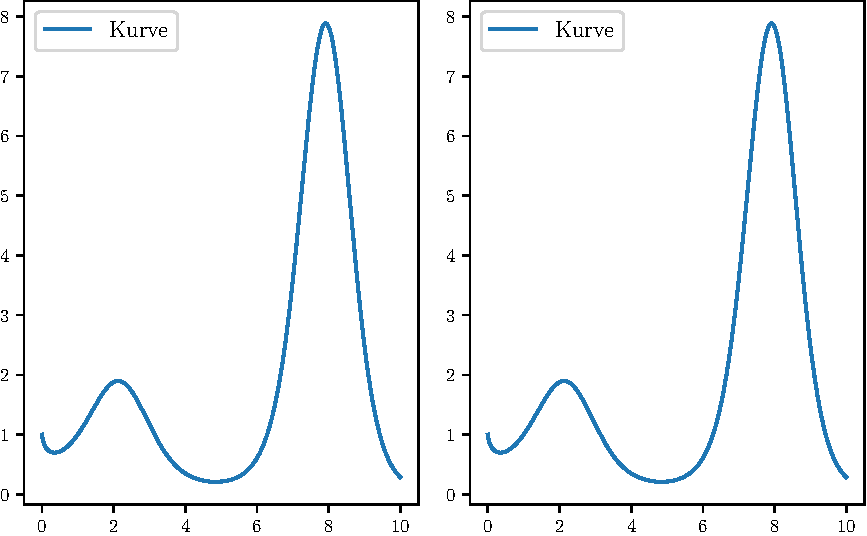
\includegraphics{plot.pdf}
  \caption{Plot.}
  \label{fig:plot}
\end{figure}
\subsection{Messung 1-15 Bar}
\begin{table}
  \centering
  \caption{Die gemessenen Fallzeiten der Kugeln bei Raumtemperatur($20\unit{\celsius}$).}
  \begin{tabular}{cc}
    \toprule
    {$p \mathbin{/} \unit{\bar}$} &
    {$T \mathbin{/} \unit{\celsius}$} \\
    \midrule
      1 & 108 \\
      2 & 120 \\
      3 & 134 \\
      4 & 140 \\
      5 & 148 \\
      6 & 156 \\
      7 & 160 \\
      8 & 166 \\
      9 & 170 \\
      10 & 174 \\
      11 & 177 \\
      12 & 182 \\
      13 & 187 \\
      14 & 189 \\
      15 & 190 \\
    \bottomrule
  \end{tabular}
  \label{tab:Tabelle2}
\end{table}
